\documentclass[border=6pt]{standalone}
\usepackage[T1]{fontenc}
\usepackage{courier}
\usepackage[scaled=0.95]{helvet}
\renewcommand{\familydefault}{\sfdefault}
\usepackage{sfmath}
\usepackage[version=4]{mhchem}
\usepackage{tikz}
\usepackage{pgfplots}
\pgfplotsset{compat=newest}
\usetikzlibrary{arrows.meta,positioning,calc,fit,backgrounds,shapes.geometric,decorations.pathreplacing,patterns}
\definecolor{ink}{HTML}{17233A}
\definecolor{inksoft}{HTML}{44506A}
\definecolor{teal}{HTML}{0E6B6B}
\definecolor{tealsoft}{HTML}{E5F0EF}
\definecolor{amber}{HTML}{B26B12}
\definecolor{ambersoft}{HTML}{FBF0DF}
\definecolor{blue}{HTML}{2F6690}
\definecolor{bluesoft}{HTML}{E3ECF4}
\definecolor{plum}{HTML}{7A4D8C}
\definecolor{plumsoft}{HTML}{EFE7F3}
\definecolor{greyc}{HTML}{8A94A3}
\definecolor{linec}{HTML}{D3DCE1}
\definecolor{oxy}{HTML}{C0392B}
\definecolor{carb}{HTML}{3B4252}
\definecolor{hyd}{HTML}{E6E9EE}
\definecolor{nit}{HTML}{2F6690}
\tikzset{
  every picture/.style={line cap=round,line join=round},
  lab/.style={font=\small, text=inksoft},
  >={Stealth[length=7pt]},
}
\pgfplotsset{
  every axis/.append style={axis line style={inksoft}, tick style={inksoft}, tick label style={font=\footnotesize, text=inksoft}, label style={font=\small, text=ink}},
}
% fragment tile: \frag{node name}{position}{colour}{content}
\newcommand{\frag}[4]{\node[draw=#3, fill=#3!12, line width=1.4pt, rounded corners=6pt, minimum width=1.25cm, minimum height=1.05cm, text=#3, font=\bfseries] (#1) at (#2) {#4};}
\newcommand{\ring}{\tikz[baseline=-0.6ex]{\draw[line width=1.1pt] (0:0.3)--(60:0.3)--(120:0.3)--(180:0.3)--(240:0.3)--(300:0.3)--cycle; \draw[line width=0.8pt] (0,0) circle (0.16);}}
\newcommand{\bond}[2]{\draw[ink, line width=2.2pt] (#1) -- (#2);}

\begin{document}
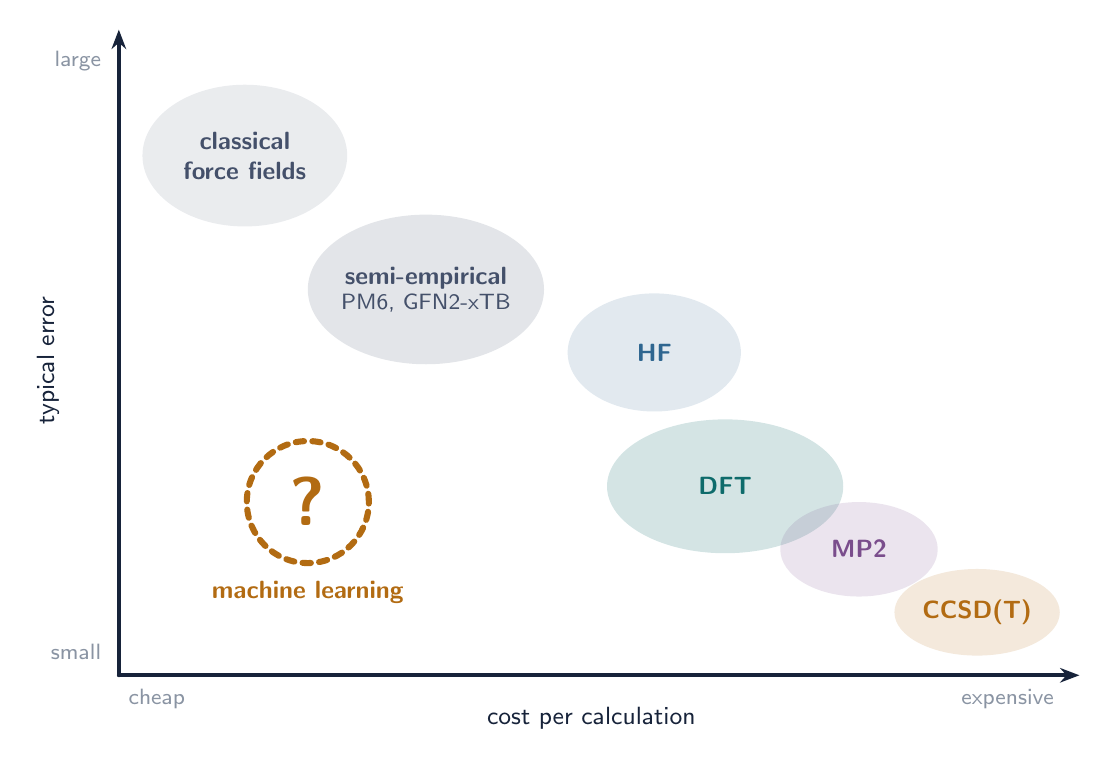
\begin{tikzpicture}
\draw[->, ink, line width=1.4pt] (0,0) -- (12.2,0); \node[font=\small, text=ink] at (6,-0.55) {cost per calculation};
\draw[->, ink, line width=1.4pt] (0,0) -- (0,8.2);
\node[font=\small, text=ink, rotate=90] at (-0.9,4.0) {typical error};
\node[font=\footnotesize, text=greyc, anchor=north west] at (0,-0.05) {cheap};
\node[font=\footnotesize, text=greyc, anchor=north east] at (12,-0.05) {expensive};
\node[font=\footnotesize, text=greyc, anchor=east] at (-0.1,0.3) {small};
\node[font=\footnotesize, text=greyc, anchor=east] at (-0.1,7.8) {large};
\fill[greyc, fill opacity=0.18] (1.6,6.6) ellipse (1.3 and 0.9); \node[font=\small\bfseries, text=inksoft, align=center] at (1.6,6.6) {classical\\force fields};
\fill[inksoft, fill opacity=0.15] (3.9,4.9) ellipse (1.5 and 0.95); \node[font=\small\bfseries, text=inksoft, align=center] at (3.9,4.9) {semi-empirical\\[-2pt]{\footnotesize\mdseries PM6, GFN2-xTB}};
\fill[blue, fill opacity=0.14] (6.8,4.1) ellipse (1.1 and 0.75); \node[font=\small\bfseries, text=blue] at (6.8,4.1) {HF};
\fill[teal, fill opacity=0.18] (7.7,2.4) ellipse (1.5 and 0.85); \node[font=\small\bfseries, text=teal] at (7.7,2.4) {DFT};
\fill[plum, fill opacity=0.15] (9.4,1.6) ellipse (1.0 and 0.6); \node[font=\small\bfseries, text=plum] at (9.4,1.6) {MP2};
\fill[amber, fill opacity=0.15] (10.9,0.8) ellipse (1.05 and 0.55); \node[font=\small\bfseries, text=amber] at (10.9,0.8) {CCSD(T)};
\node[circle, draw=amber, line width=2.2pt, dashed, minimum size=1.55cm, font=\fontsize{34}{34}\selectfont\bfseries, text=amber, fill=white] at (2.4,2.2) {?};
\node[font=\small\bfseries, text=amber] at (2.4,1.05) {machine learning};
\end{tikzpicture}
\end{document}
